\begin{myQA}{编译到 \filename{eu1lmr.fd} 时很慢怎么办?}
据说,只有在 Windows 系统上用 \hologo{XeTeX} 编译时才会出现这种情况。
\hologo{XeTeX} 会调用系统字体,安装新字体后,需要刷新字体缓存,
以使 \hologo{XeTeX} 识别新安装的字体。
可以使用 \code|fc-cache -f| 命令来重建字体缓存。

关于 \code|fc-cache| 更多用法,可以输入 \code|fc-cache --help| 来查看。

在 Mac 上,由于不使用 \filename{fontconfig} 机制,
因此不会出现该问题。

\myRef{\citet{TSE2015eu1lmr}}
\end{myQA}

%\begin{myQA}{cmbright 字体为什么有锯齿?}
%	因为
%\end{myQA}

\begin{myQA}{如何使用好看的数学字体?}
\TeX 和 \LaTeX 的默认字体是高老爷子制作的 Computer Modern,
如图~\ref{Fig:cm_1} 所示。
%	\begin{equation*}
%		\int\sin^2 x \,\mathrm{d} x
%		=\frac{1}{2}x - \frac{1}{4} \sin 2x + C
%	\end{equation*}

\begin{figure}[h]
	\centering
	\framebox{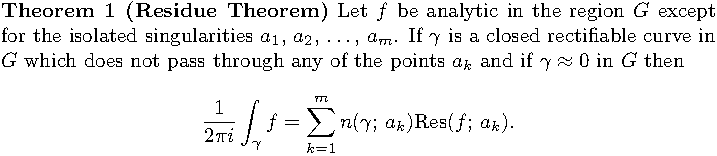
\includegraphics{Examples/cm_1}}
	\caption{Computer Modern 字体示例}
	\label{Fig:cm_1}
\end{figure}

好看是好看,但是多了也觉得乏味。下面推荐几个字体宏包,给诸位换换口味。

首先是 CM Bright(图~\ref{Fig:cmbright}),这是一个能与
Computer Modern 相配的无衬线字体,
包含在 \pkg{cmbright} \indexpkg{cmbright}宏包中。

CM Birght 不包含积分、求和等巨算符,默认采用
Computer Modern 代替,处女座自是不会满意。不过稍费工夫,
也有办法改用其他字体(Iwona 之类)。
%TODO:20160827 需要引用其他问题

\begin{figure}[h]
	\centering
	\framebox{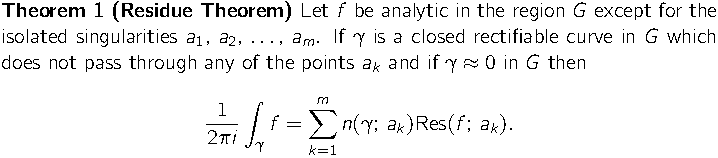
\includegraphics{Examples/cmbright}}
	\caption{CM Bright 字体示例}
	\label{Fig:cmbright}
\end{figure}

接下来是烂大街的 Times 系列(图~\ref{Fig:txfonts})。
这里的例子是效果比较好的 \pkg{txfonts} \indexpkg{txfonts} 宏包,
也可以用 \pkg{mathptm} \indexpkg{mathptm} 或者
\pkg{mathptmx} \indexpkg{mathptmx} 宏包代替。

请注意,这里所谓“Times”字体并非专指 Times New Roman。
这几个宏包用的是 URW Nimbus Roman No. 9 L,这是一个开源字体。
%TODO:20160828 newtxmath

\begin{figure}[h]
	\centering
	\framebox{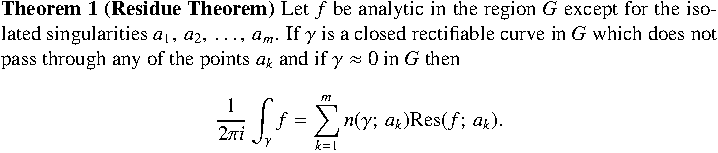
\includegraphics{Examples/txfonts}}
	\caption{Times 字体示例(\pkg{txfonts} 宏包)}
	\label{Fig:txfonts}
\end{figure}

然后是与 \pkg{txfonts} 系出同门的 \pkg{pxfonts}
\indexpkg{pxfonts} 宏包(图~\ref{Fig:pxfonts}),
它提供了完整的 Palatino 字体方案。实际用的字体是 URW Palladio L。

\begin{figure}[h]
	\centering
	\framebox{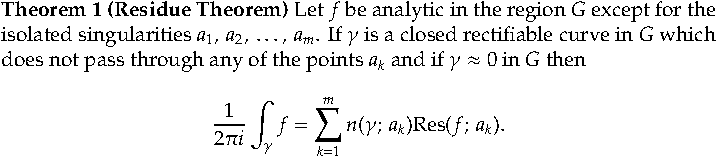
\includegraphics{Examples/pxfonts}}
	\caption{Palatino 字体示例(\pkg{pxfonts} 宏包)}
	\label{Fig:pxfonts}
\end{figure}

以上几个字体包都是久经考验且方便易用的:
直接在导言区加上 \code|\usepackage{*|\optional{宏包名}|*}|
就可以获得理想的效果。
\end{myQA}

\begin{myQA}{如何使用更好看的数学字体?}
\end{myQA}